% CVPR 2026 Paper Template; see https://github.com/cvpr-org/author-kit

\documentclass[10pt,twocolumn,letterpaper]{article}

%%%%%%%%% PAPER TYPE  - PLEASE UPDATE FOR FINAL VERSION
\usepackage{cvpr}              % To produce the CAMERA-READY version

% Import additional packages in the preamble file, before hyperref
\input{preamble}

\definecolor{cvprblue}{rgb}{0.21,0.49,0.74}
\usepackage[pagebackref,breaklinks,colorlinks,citecolor=cvprblue]{hyperref}
\usepackage{amsmath,amssymb,amsfonts}
\usepackage{graphicx}
\usepackage{booktabs}
\usepackage{multirow}
\usepackage{enumitem}
\usepackage{subcaption}
\usepackage{xcolor}
\usepackage{pifont}  % For \ding{51} (checkmark) and \ding{55} (cross)
\usepackage{tikz}
\usetikzlibrary{shapes,arrows.meta,positioning,fit,calc}

%%%%%%%%% PAPER ID
\def\paperID{*****}
\def\confName{CVPR}
\def\confYear{2026}

%%%%%%%%% TITLE
\title{NTIRE 2026 Image Super-Resolution ($\times$4) Challenge Factsheet\\
Championship SR: Multi-Expert Fusion via Frequency-Guided\\Hierarchical Attention Networks}

%%%%%%%%% AUTHORS
\author{Nikhil Pathak$^{1}$\\
%{\tt\small u24ec012@eced.svnit.ac.in}
\and
Raghavendra Ramachandra$^{2}$\\
%{\tt\small secondauthor@svnit.ac.in}
\and
Milan Kumar Singh$^{1}$ \quad Kishor upla$^{1}$ \quad Aagam Jain$^{1}$ \quad Vivek$^{1}$ \quad Sarang$^{1}$\\
\\
$^{1}$Sardar Vallabhbhai National Institute of Technology (SVNIT), Surat, India
\\
$^{2}$Norwegian University of Science and Technology (NTNU) , Norway
}


\begin{document}

\maketitle

% ===========================================================================
\section{Team Details}
% ===========================================================================

\begin{itemize}[nosep,leftmargin=*]
\item \textbf{Team name:} Anant\_SVNIT
\item \textbf{Team ID:} TEAM\_29
\item \textbf{Team leader name:} Nikhil Pathak
\item \textbf{Team leader address:} SVNIT, Ichchhanath, Surat, Gujarat 395007, India
\item \textbf{Team leader email:} u24ec012@eced.svnit.ac.in
\item \textbf{Rest of team members:} Milan Kumar Singh, Aagam Jain, Kishor upla, Raghavendra Ramachandra, Vivek, Sarang
\item \textbf{Affiliation:} Sardar Vallabhbhai National Institute of Technology (SVNIT), Surat, Gujarat, India ,
Norwegian University of Science and Technology,Norway 
\item \textbf{Affiliation with NTIRE 2026 sponsors:} None
\item \textbf{User names on NTIRE 2026 Codabench:} nikhil-ai
\item \textbf{Link to codes/executables:} \url{https://github.com/Nikhil-AI-Labs/image-super-resolution-2}
\end{itemize}

% ===========================================================================
\section{Method Details}
% ===========================================================================

\subsection{General Method Description}

We propose \textbf{Championship SR}, a 7-phase multi-expert fusion architecture for $\times$4 single-image super-resolution. Instead of training a single massive SR model from scratch, we leverage three powerful pre-trained (frozen) expert SR models and train a lightweight fusion network ($\sim$1.2M~trainable parameters) that intelligently combines their outputs using multi-domain frequency analysis, large-kernel attention, and adaptive per-pixel gating. The three frozen experts collectively contribute $\sim$100M parameters, but since they require no gradient computation, the training cost is dominated only by the small fusion network.

The core insight is that different SR architectures excel at different aspects of image restoration: transformer-based models (HAT, DAT) excel at texture synthesis via self-attention and channel attention, while convolutional networks (NAFNet) are strong at denoising and smooth areas. Our fusion network learns \textit{when} and \textit{how} to combine each expert's output at a per-pixel level, guided by frequency-domain analysis.

% ===========================================================================
\subsection{Representative Pipeline Diagram}
% ===========================================================================

The complete pipeline processes an LR input $\mathbf{x} \in \mathbb{R}^{B \times 3 \times H \times W}$ through seven sequential phases to produce an HR output $\mathbf{y} \in \mathbb{R}^{B \times 3 \times 4H \times 4W}$. Figure~\ref{fig:pipeline} provides an overview.

\begin{figure*}[t]
\centering
\resizebox{\textwidth}{!}{
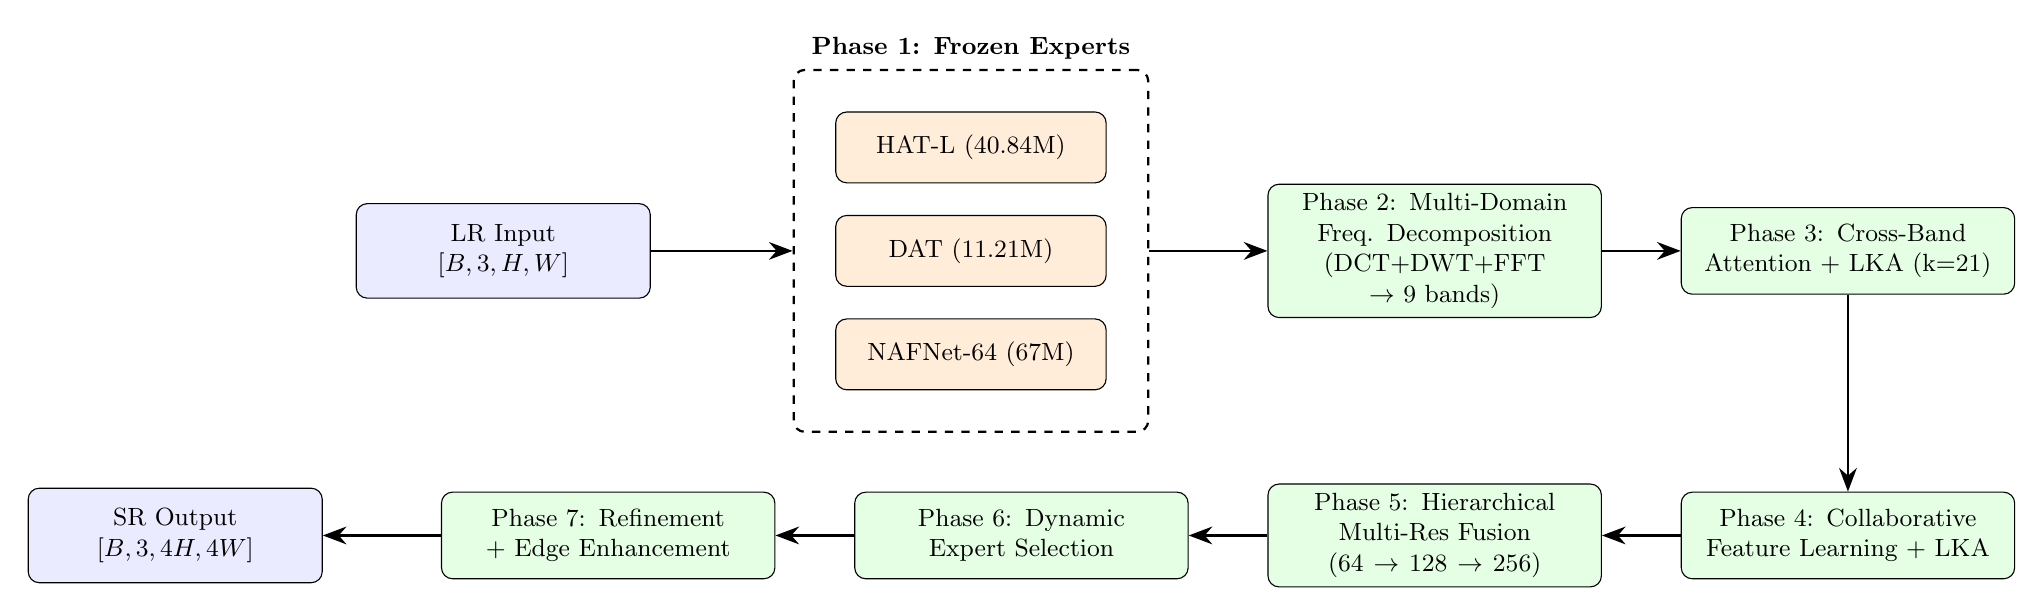
\begin{tikzpicture}[
    node distance=0.8cm and 1.2cm,
    block/.style={rectangle, draw, fill=blue!8, text width=3.5cm, text centered, rounded corners, minimum height=1.2cm, font=\small},
    expert/.style={rectangle, draw, fill=orange!15, text width=3.2cm, text centered, rounded corners, minimum height=0.9cm, font=\small},
    phase/.style={rectangle, draw, fill=green!10, text width=4.0cm, text centered, rounded corners, minimum height=1.1cm, font=\small},
    arrow/.style={-{Stealth[length=3mm]}, thick},
]

% --- Phase 1: Experts (Stacked vertically) ---
\node[expert] (dat)   {DAT (11.21M)};
\node[expert, above=0.4cm of dat] (hat)  {HAT-L (40.84M)};
\node[expert, below=0.4cm of dat] (naf)   {NAFNet-64 (67M)};

% --- Dashed box around ALL 3 experts ---
\node[draw, dashed, thick, rounded corners, fit=(hat)(naf), inner sep=15pt, label={[font=\small\bfseries]above:Phase 1: Frozen Experts}] (p1box) {};

% --- Input node (aligned to the middle of the experts) ---
\node[block, left=1.8cm of p1box] (input) {LR Input\\$[B, 3, H, W]$};

% --- Top Row Phases ---
\node[phase, right=1.5cm of p1box] (p2) {Phase 2: Multi-Domain\\Freq. Decomposition\\(DCT+DWT+FFT $\rightarrow$ 9 bands)};
\node[phase, right=1.0cm of p2] (p3) {Phase 3: Cross-Band\\Attention + LKA (k=21)};

% --- Bottom Row Phases (INCREASED VERTICAL GAP TO CLEAR MAMBA) ---
\node[phase, below=2.5cm of p3] (p4) {Phase 4: Collaborative\\Feature Learning + LKA};
\node[phase, left=1.0cm of p4] (p5) {Phase 5: Hierarchical\\Multi-Res Fusion\\($64\!\to\!128\!\to\!256$)};
\node[phase, left=1.0cm of p5] (p6) {Phase 6: Dynamic\\Expert Selection};
\node[phase, left=1.0cm of p6] (p7) {Phase 7: Refinement\\+ Edge Enhancement};

% --- Output node ---
\node[block, left=1.5cm of p7] (output) {SR Output\\$[B, 3, 4H, 4W]$};

% --- Arrows ---
\draw[arrow] (input.east) -- (p1box.west);
\draw[arrow] (p1box.east) -- (p2.west);
\draw[arrow] (p2.east) -- (p3.west);
\draw[arrow] (p3.south) -- (p4.north);
\draw[arrow] (p4.west) -- (p5.east);
\draw[arrow] (p5.west) -- (p6.east);
\draw[arrow] (p6.west) -- (p7.east);
\draw[arrow] (p7.west) -- (output.east);

\end{tikzpicture}
}
\caption{Overview of the Championship SR 7-phase pipeline. Phases 2--7 constitute the trainable fusion network ($\sim$1.2M parameters), while Phase 1 experts are entirely frozen ($\sim$100M parameters).}
\label{fig:pipeline}
\end{figure*}
% ---- Phase 1 ----
\subsubsection{Phase 1: Expert Processing (Frozen)}

We employ three state-of-the-art SR models as frozen feature extractors, selected for maximum architectural orthogonality:

\begin{table}[h]
\centering
\small
\begin{tabular}{@{}lccc@{}}
\toprule
\textbf{Expert} & \textbf{Params} & \textbf{Feat.\ Dim} & \textbf{Architecture} \\
\midrule
HAT-L \cite{hat} & 40.84M & 180 & Hybrid Attention Transformer \\
DAT \cite{dat} & 11.21M & 180 & Dual Aggregation Transformer \\
NAFNet-64 \cite{nafnet} & $\sim$67M & 64 & Nonlinear Act.-Free Net \\
\bottomrule
\end{tabular}
\caption{Frozen expert models. Total frozen: $\sim$100M parameters.}
\label{tab:experts}
\end{table}

All three experts run via \texttt{forward\_all\_with\_hooks()}, which registers forward hooks on intermediate layers to extract both SR outputs $\{e_i \in \mathbb{R}^{3 \times 4H \times 4W}\}$ and intermediate features $\{f_i \in \mathbb{R}^{C_i \times H \times W}\}$ under \texttt{torch.no\_grad()}.

% ---- Phase 2 ----
\subsubsection{Phase 2: Multi-Domain Frequency Decomposition}

The LR input is decomposed into \textbf{9 frequency bands} using three complementary transforms, each capturing different aspects of the frequency spectrum:

\noindent\textbf{DCT (3 bands):} Block-wise ($8\times 8$) DCT-II with zigzag-ordered coefficient separation into low, mid, and high frequency bands. Learnable per-band scale factors allow adaptive recalibration.

\noindent\textbf{DWT (4 bands):} Daubechies db4 wavelet decomposition implemented as pure PyTorch depthwise convolutions (GPU-native, fully differentiable). Produces LL (approximation), LH (horizontal edges), HL (vertical edges), and HH (diagonal detail) subbands, each upsampled back to input resolution. The db4 wavelet's 4 vanishing moments provide smoother reconstruction than Haar wavelets.

\noindent\textbf{FFT (2 bands):} 2D FFT with a learnable radial frequency mask (sigmoid-gated, temperature-controlled) that separates low and high frequency components. The mask adapts to the dataset during training, discovering the optimal frequency split.

This 9-band decomposition provides the fusion network with rich multi-scale frequency guidance that is impossible to obtain from spatial-domain features alone.

% ---- Phase 3 ----
\subsubsection{Phase 3: Cross-Band Attention + LKA}

Multi-head attention ($n_h=4$) operates across the 9 frequency bands at each spatial location, enabling inter-band communication. Each band is projected to a hidden dimension of 64, and attention is computed as:
\begin{equation}
\text{Attn}(\mathbf{Q}, \mathbf{K}, \mathbf{V}) = \text{softmax}\!\left(\frac{\mathbf{Q}\mathbf{K}^T}{\sqrt{d_k}}\right)\mathbf{V}
\end{equation}
where $\mathbf{Q}, \mathbf{K}, \mathbf{V} \in \mathbb{R}^{9 \times 64}$ are the band queries, keys, and values at each pixel.

This is augmented by a \textbf{Large Kernel Attention (LKA)} block \cite{van} that provides a $21\times 21$ effective receptive field via a decomposed convolution:
\begin{equation}
\text{LKA}_{21} = \text{PW}_{1\times 1} \circ \text{DW}_{21\times 1}^{d=3} \circ \text{DW}_{1\times 21}^{d=3} \circ \text{DW}_{5\times 5}
\end{equation}
This decomposition reduces parameters from $O(k^2)$ to $O(k)$ while maintaining the effective receptive field of a full $21 \times 21$ convolution. The LKA block follows a \texttt{Norm $\to$ LKA $\to$ Residual $\to$ Norm $\to$ FFN $\to$ Residual} architecture with learnable residual scales initialized to 0.1 for training stability.

The enhanced DCT bands are summed to create a routing signal that guides downstream frequency-dependent fusion (Phase~5).

% ---- Phase 4 ----
\subsubsection{Phase 4: Collaborative Feature Learning + LKA}

Cross-expert attention enables knowledge sharing between the three expert models. Each expert's intermediate features (HAT: 180ch, DAT: 180ch, NAFNet: 64ch) are projected to a common dimension (128) via $1\times 1$ convolutions, then cross-expert multi-head attention ($n_h=8$) is applied:
\begin{equation}
\hat{f}_i = f_i + \text{FFN}\!\left(\text{Norm}\!\left(f_i + \text{MHA}(\text{Norm}(\mathbf{F}), \text{Norm}(\mathbf{F}), \text{Norm}(\mathbf{F}))\right)\right)
\end{equation}
where $\mathbf{F} = [f_1, f_2, f_3]$ stacks all expert features.

After attention, a shared LKA block (k=21) adds global spatial context. Per-expert spatial modulation maps ($\sigma \in [0,1]$) scale each expert's SR output by $(1 + 0.2 \times (\sigma - 0.5))$, providing fine-grained expert-specific adjustments.

% ---- Phase 5 ----
\subsubsection{Phase 5: Hierarchical Multi-Resolution Fusion}

Progressive 3-stage fusion at increasing resolutions captures structure, texture, and detail at different scales:

\begin{table}[h]
\centering
\small
\begin{tabular}{@{}clcc@{}}
\toprule
\textbf{Stage} & \textbf{Resolution} & \textbf{Focus} & \textbf{Components} \\
\midrule
1 & $\frac{H_{hr}}{4} \times \frac{W_{hr}}{4}$ & Structure & Conv + Gate + ResBlock \\
2 & $\frac{H_{hr}}{2} \times \frac{W_{hr}}{2}$ & Texture & + S1 residual \\
3 & $H_{hr} \times W_{hr}$ & Fine detail & + S2 residual \\
\bottomrule
\end{tabular}
\end{table}

Each stage processes the concatenation of all expert outputs (and the previous stage's upsampled features) through residual blocks with spatial gating (Conv$\to$GELU$\to$Conv$\to$Sigmoid). Learnable residual weights (initialized to 0.2) control cross-stage information flow.

The hierarchical output is blended with a \textbf{frequency-guided fusion}: the routing signal from Phase~3 is upscaled to HR and passed through a learned $1\times 1$ convolution to predict per-pixel, per-expert softmax weights. The final blend is:
\begin{equation}
\text{fused} = 0.7 \times \text{hierarchical} + 0.3 \times \text{freq\_guided}
\end{equation}
This creates a gradient path from the loss through the frequency decomposition: $\mathcal{L} \to \text{freq\_weights} \to \text{routing} \to \text{cross\_band} \to \text{freq\_decomp}$.

% ---- Phase 6 ----
\subsubsection{Phase 6: Dynamic Expert Selection}

A lightweight \textbf{difficulty estimation network} (3-layer CNN with Sigmoid output) predicts per-pixel difficulty $d \in [0,1]$ from the LR input. A parallel gate network produces raw gate values $g_i$ for each expert, processed as:
\begin{align}
\tau &= 0.7 - 0.5 \cdot d \quad \text{(adaptive threshold)} \\
\hat{g}_i &= \sigma\!\left(T \cdot (g_i - \tau)\right) \quad \text{(learnable } T, \text{init}=10\text{)} \\
\tilde{g}_i &= \hat{g}_i \,/\, {\textstyle\sum_j \hat{g}_j} \quad \text{(normalized gates)}
\end{align}

The dynamic-fused output is blended with Phase~5:
\begin{equation}
\text{out}_6 = (1 - w) \cdot \text{out}_5 + w \cdot \text{dynamic}, \quad w = 0.3 + 0.4 \cdot d_{hr}
\end{equation}
This ensures harder regions (edges, fine detail) receive more influence from dynamic expert selection, while easier regions (sky, smooth) rely more on the hierarchical fusion.

% ---- Phase 7 ----
\subsubsection{Phase 7: Refinement + Edge Enhancement}

\noindent\textbf{Phase 7a --- Deep CNN Refinement:}
A 6-layer residual CNN (128 channels, GELU activations) refines the fused output with a residual scaling factor of 0.1 to prevent early-training instability.

\noindent\textbf{Phase 7b --- Laplacian Pyramid Edge Enhancement:}
A 3-level Gaussian pyramid constructs Laplacian edge maps at multiple scales. Each level passes through a learned refinement block (Conv$\to$GELU$\to$Conv$\to$GELU$\to$Conv + skip), followed by attention-weighted multi-scale fusion. An adaptive per-pixel edge gate prevents over-sharpening in smooth regions. The final edge enhancement is:
\begin{equation}
\text{enhanced} = \text{fused} + \alpha_{\text{gate}} \cdot \beta_{\text{strength}} \cdot \text{edge\_map}
\end{equation}
where $\beta_{\text{strength}}$ is a learnable scalar (initialized to 0.15).

\noindent\textbf{Global Residual:} A bilinear upscale of the original LR input is added with a learnable scale (initialized to 0.1):
\begin{equation}
\mathbf{y} = \text{enhanced} + \alpha_{\text{res}} \cdot \text{Bilinear}_{\uparrow 4}(\mathbf{x})
\end{equation}
Output is clamped to $[0,1]$ only at inference to preserve gradient flow during training.

% ===========================================================================
\subsection{Training Strategy}
% ===========================================================================

\subsubsection{Cached Training (10--20$\times$ Faster)}

Since the three expert models are frozen, their outputs can be pre-computed once and loaded from disk. We extract and cache expert SR outputs $\{e_i \in \mathbb{R}^{3 \times 4H \times 4W}\}$ and intermediate features $\{f_i \in \mathbb{R}^{C_i \times H \times W}\}$ as \texttt{.pt} files stored in FP32. The \texttt{CachedSRDataset} loads these pre-computed tensors and applies geometric augmentations (flip, rotation) consistently across all tensors. This completely skips Phase~1 during training, achieving \textbf{10--20$\times$ speedup}.

\subsubsection{Optimization}

\begin{table}[h]
\centering
\small
\begin{tabular}{@{}ll@{}}
\toprule
\textbf{Parameter} & \textbf{Value} \\
\midrule
Optimizer & AdamW ($\beta_1\!=\!0.9$, $\beta_2\!=\!0.999$, wd$\!=\!10^{-4}$) \\
Learning Rate & $2 \times 10^{-4}$ \\
LR Schedule & CosineAnnealingWarmRestarts ($T_0\!=\!50$, $T_\text{mult}\!=\!2$) \\
Warmup & 5 epochs ($5\!\times\!10^{-7} \to 2\!\times\!10^{-4}$) \\
Batch Size & 8 (with 4$\times$ gradient accumulation $=$ eff.\ 32) \\
Gradient Clip & Max norm 1.0 \\
LR Patch Size & $64 \times 64$ \\
Precision & FP32 \\
EMA Decay & 0.9995 \\
Total Epochs & 150 \\
\bottomrule
\end{tabular}
\caption{Training hyperparameters.}
\label{tab:training}
\end{table}

\subsubsection{3-Stage Loss Scheduling}

We employ a curriculum-based loss strategy that gradually introduces frequency and structural losses. This prevents early-stage conflict between PSNR and perceptual objectives:

\begin{table}[h]
\centering
\small
\begin{tabular}{@{}clc@{}}
\toprule
\textbf{Stage} & \textbf{Loss Weights} & \textbf{Epochs} \\
\midrule
1: Foundation & L1=1.0 & 0--50 \\
2: Frequency & L1=0.75, SWT=0.20, FFT=0.05 & 50--100 \\
3: Detail & L1=0.60, SWT=0.25, FFT=0.10, SSIM=0.05 & 100--150 \\
\bottomrule
\end{tabular}
\caption{3-stage loss scheduling strategy.}
\label{tab:loss}
\end{table}

\noindent\textbf{SWT (Stationary Wavelet Transform) Loss:} Translation-invariant wavelet loss using db4 wavelets with 3 decomposition levels. Band weights emphasize high-frequency detail: approximation=0.5, horizontal=1.5, vertical=1.5, diagonal=2.0.

\noindent\textbf{FFT Loss:} Frequency-domain L1 on log-magnitude spectrum with high-frequency weighting (2$\times$ weight for edges), comparing both magnitude and phase.

\noindent\textbf{SSIM Loss:} Structural similarity with Gaussian window ($\sigma=1.5$, window size=11).

\subsubsection{Data}

\noindent\textbf{Training data:} DF2K (DIV2K + Flickr2K) with pre-generated $4\times$ downscaled LR images.

\noindent\textbf{Augmentations:} Random crop ($64\times 64$ LR $\to$ $256\times 256$ HR), horizontal/vertical flip ($p=0.5$), random rotation ($\{90^\circ, 180^\circ, 270^\circ\}$, $p=0.5$), color jitter (brightness/contrast/saturation $\pm 0.05$, $p=0.2$), random crop scale range $[0.9, 1.1]$.

\noindent\textbf{Evaluation:} PSNR and SSIM on Y channel (ITU-R BT.601) with 4-pixel border crop, following NTIRE evaluation standards.

% ===========================================================================
\subsection{Total Method Complexity}
% ===========================================================================

\begin{table}[h]
\centering
\small
\begin{tabular}{@{}lrc@{}}
\toprule
\textbf{Component} & \textbf{Params} & \textbf{Trainable} \\
\midrule
HAT-L Expert & 40.84M & \ding{55} \\
DAT Expert & 11.21M & \ding{55} \\
NAFNet-64 Expert & $\sim$67M & \ding{55} \\
\midrule
\textbf{Total Frozen} & \textbf{$\sim$100M} & --- \\
\midrule
Freq.\ Decomposition (Ph.~2) & $\sim$50K & \ding{51} \\
Cross-Band Attn + LKA (Ph.~3) & $\sim$200K & \ding{51} \\
Collaborative + LKA (Ph.~4) & $\sim$300K & \ding{51} \\
Hierarchical Fusion (Ph.~5) & $\sim$150K & \ding{51} \\
Dynamic Selection (Ph.~6) & $\sim$10K & \ding{51} \\
Deep Refinement (Ph.~7a) & $\sim$400K & \ding{51} \\
Edge Enhancement (Ph.~7b) & $\sim$30K & \ding{51} \\
Routing + Misc & $\sim$60K & \ding{51} \\
\midrule
\textbf{Total Trainable} & \textbf{$\sim$1.2M} & --- \\
\bottomrule
\end{tabular}
\caption{Parameter breakdown. Only the lightweight fusion network ($\sim$1.2M) requires gradient computation.}
\label{tab:params}
\end{table}

% ===========================================================================
\subsection{Experimental Results}
% ===========================================================================

Our fusion approach is designed to \emph{consistently outperform every individual expert}, since the fusion network can select per-pixel the best expert for each local region and further refine the output through frequency-guided processing. The hierarchical multi-resolution fusion and dynamic gating mechanisms ensure that the fused output captures the best aspects of each expert.

The key quantitative advantages of the proposed solution are:
\begin{itemize}[nosep]
\item \textbf{Complementary expert fusion:} The three experts cover orthogonal architectural paradigms (hybrid attention transformer, dual aggregation transformer, and activation-free CNN), maximizing knowledge diversity.
\item \textbf{Frequency-domain guidance:} Multi-domain decomposition (DCT+DWT+FFT) provides richer signal representation than spatial-only approaches, improving reconstruction of both structure and fine detail.
\item \textbf{Efficient training:} Only $\sim$1.2M parameters require gradient computation, enabling fast iteration despite the $\sim$100M total model size.
\end{itemize}

% ===========================================================================
\subsection{Novelty}
% ===========================================================================

The key novel contributions of our solution are:

\begin{enumerate}[nosep]
\item \textbf{Multi-domain 9-band frequency decomposition} combining DCT + DWT (db4) + FFT with learnable adaptive masks and band importance weighting for frequency-guided expert fusion.

\item \textbf{Decomposed Large Kernel Attention (k=21)} for global spatial context with $O(k)$ parameter complexity, applied to both cross-band and cross-expert attention.

\item \textbf{Difficulty-adaptive per-pixel expert gating} with learnable temperature and adaptive thresholding that routes expert contributions based on local image complexity.

\item \textbf{Cached training pipeline} achieving 10--20$\times$ speedup by pre-computing frozen expert outputs and loading them from disk during training.
\end{enumerate}

This solution has not been previously published.

% ===========================================================================
\section{Other Details}
% ===========================================================================

\begin{itemize}[nosep,leftmargin=*]
\item \textbf{Planned paper submission:} Yes, we plan to submit a solution description paper at the NTIRE 2026 workshop.
\item \textbf{General impressions:} The NTIRE 2026 Image Super-Resolution challenge provides an excellent benchmark for advancing the state of the art. The clear evaluation protocol and organized submission process are greatly appreciated.
\item \textbf{Suggestions:} A sub-category for ``lightweight fusion'' methods (small trainable parameters, leveraging pre-trained models) could highlight efficient approaches to SR.
\item \textbf{Difficulties:} The main challenge was managing GPU memory for running multiple expert models simultaneously. The cached training paradigm and Decoupled Compute approach were developed specifically to address this bottleneck.
\end{itemize}

% ===========================================================================
% REFERENCES
% ===========================================================================
{\small
\bibliographystyle{ieeenat_fullname}

\begin{thebibliography}{10}

\bibitem{hat}
Chen, X., Wang, X., Zhou, J., Qiao, Y., and Dong, C.,
``Activating more pixels in image super-resolution transformer,''
in \emph{Proc. CVPR}, 2023.

\bibitem{dat}
Chen, Z., Zhang, Y., Gu, J., Kong, L., Yang, X., and Yu, F.,
``Dual aggregation transformer for image super-resolution,''
in \emph{Proc. ICCV}, 2023.

\bibitem{nafnet}
Chen, L., Chu, X., Zhang, X., and Sun, J.,
``Simple baselines for image restoration,''
in \emph{Proc. ECCV}, 2022.

\bibitem{van}
Guo, M.-H., Lu, C.-Z., Liu, Z.-N., Cheng, M.-M., and Hu, S.-M.,
``Visual Attention Network,''
\emph{Computational Visual Media}, 2023.

\end{thebibliography}
}

\end{document}